\documentclass[12pt]{article}

\usepackage{graphicx} %This package allows for including figures (images) in LaTeX
%documents.
\usepackage{subfig} %This package allows you to work with subfigures.


\begin{document}

%Note that figures (and tables) are floating objects, so instead of them being
%placed exactly where you put them in the .tex document, LaTeX works out the
%best place for them to be placed in the rendered document. This is very useful,
%altough you do have the option to control this.

\begin{figure}%locations can be defined in square brackets following this
%command, either !=overrides LaTeX, h=here, t=top, b=bottom, p=special page for floating
%objects. If you leave it blank, the default is [h], meaning it will place the
%object in that location. It may not be the exact location as LaTeX will
%determine the best actual place to put it. You'd need to override LaTeX to
%achieve this, e.g. [!h].

\begin{center}
\quad %This is a separation command.
%Note that the \subfloat command is part of the subfig package.
\subfloat[Image of a cassowary]{\label{fig:bird1}
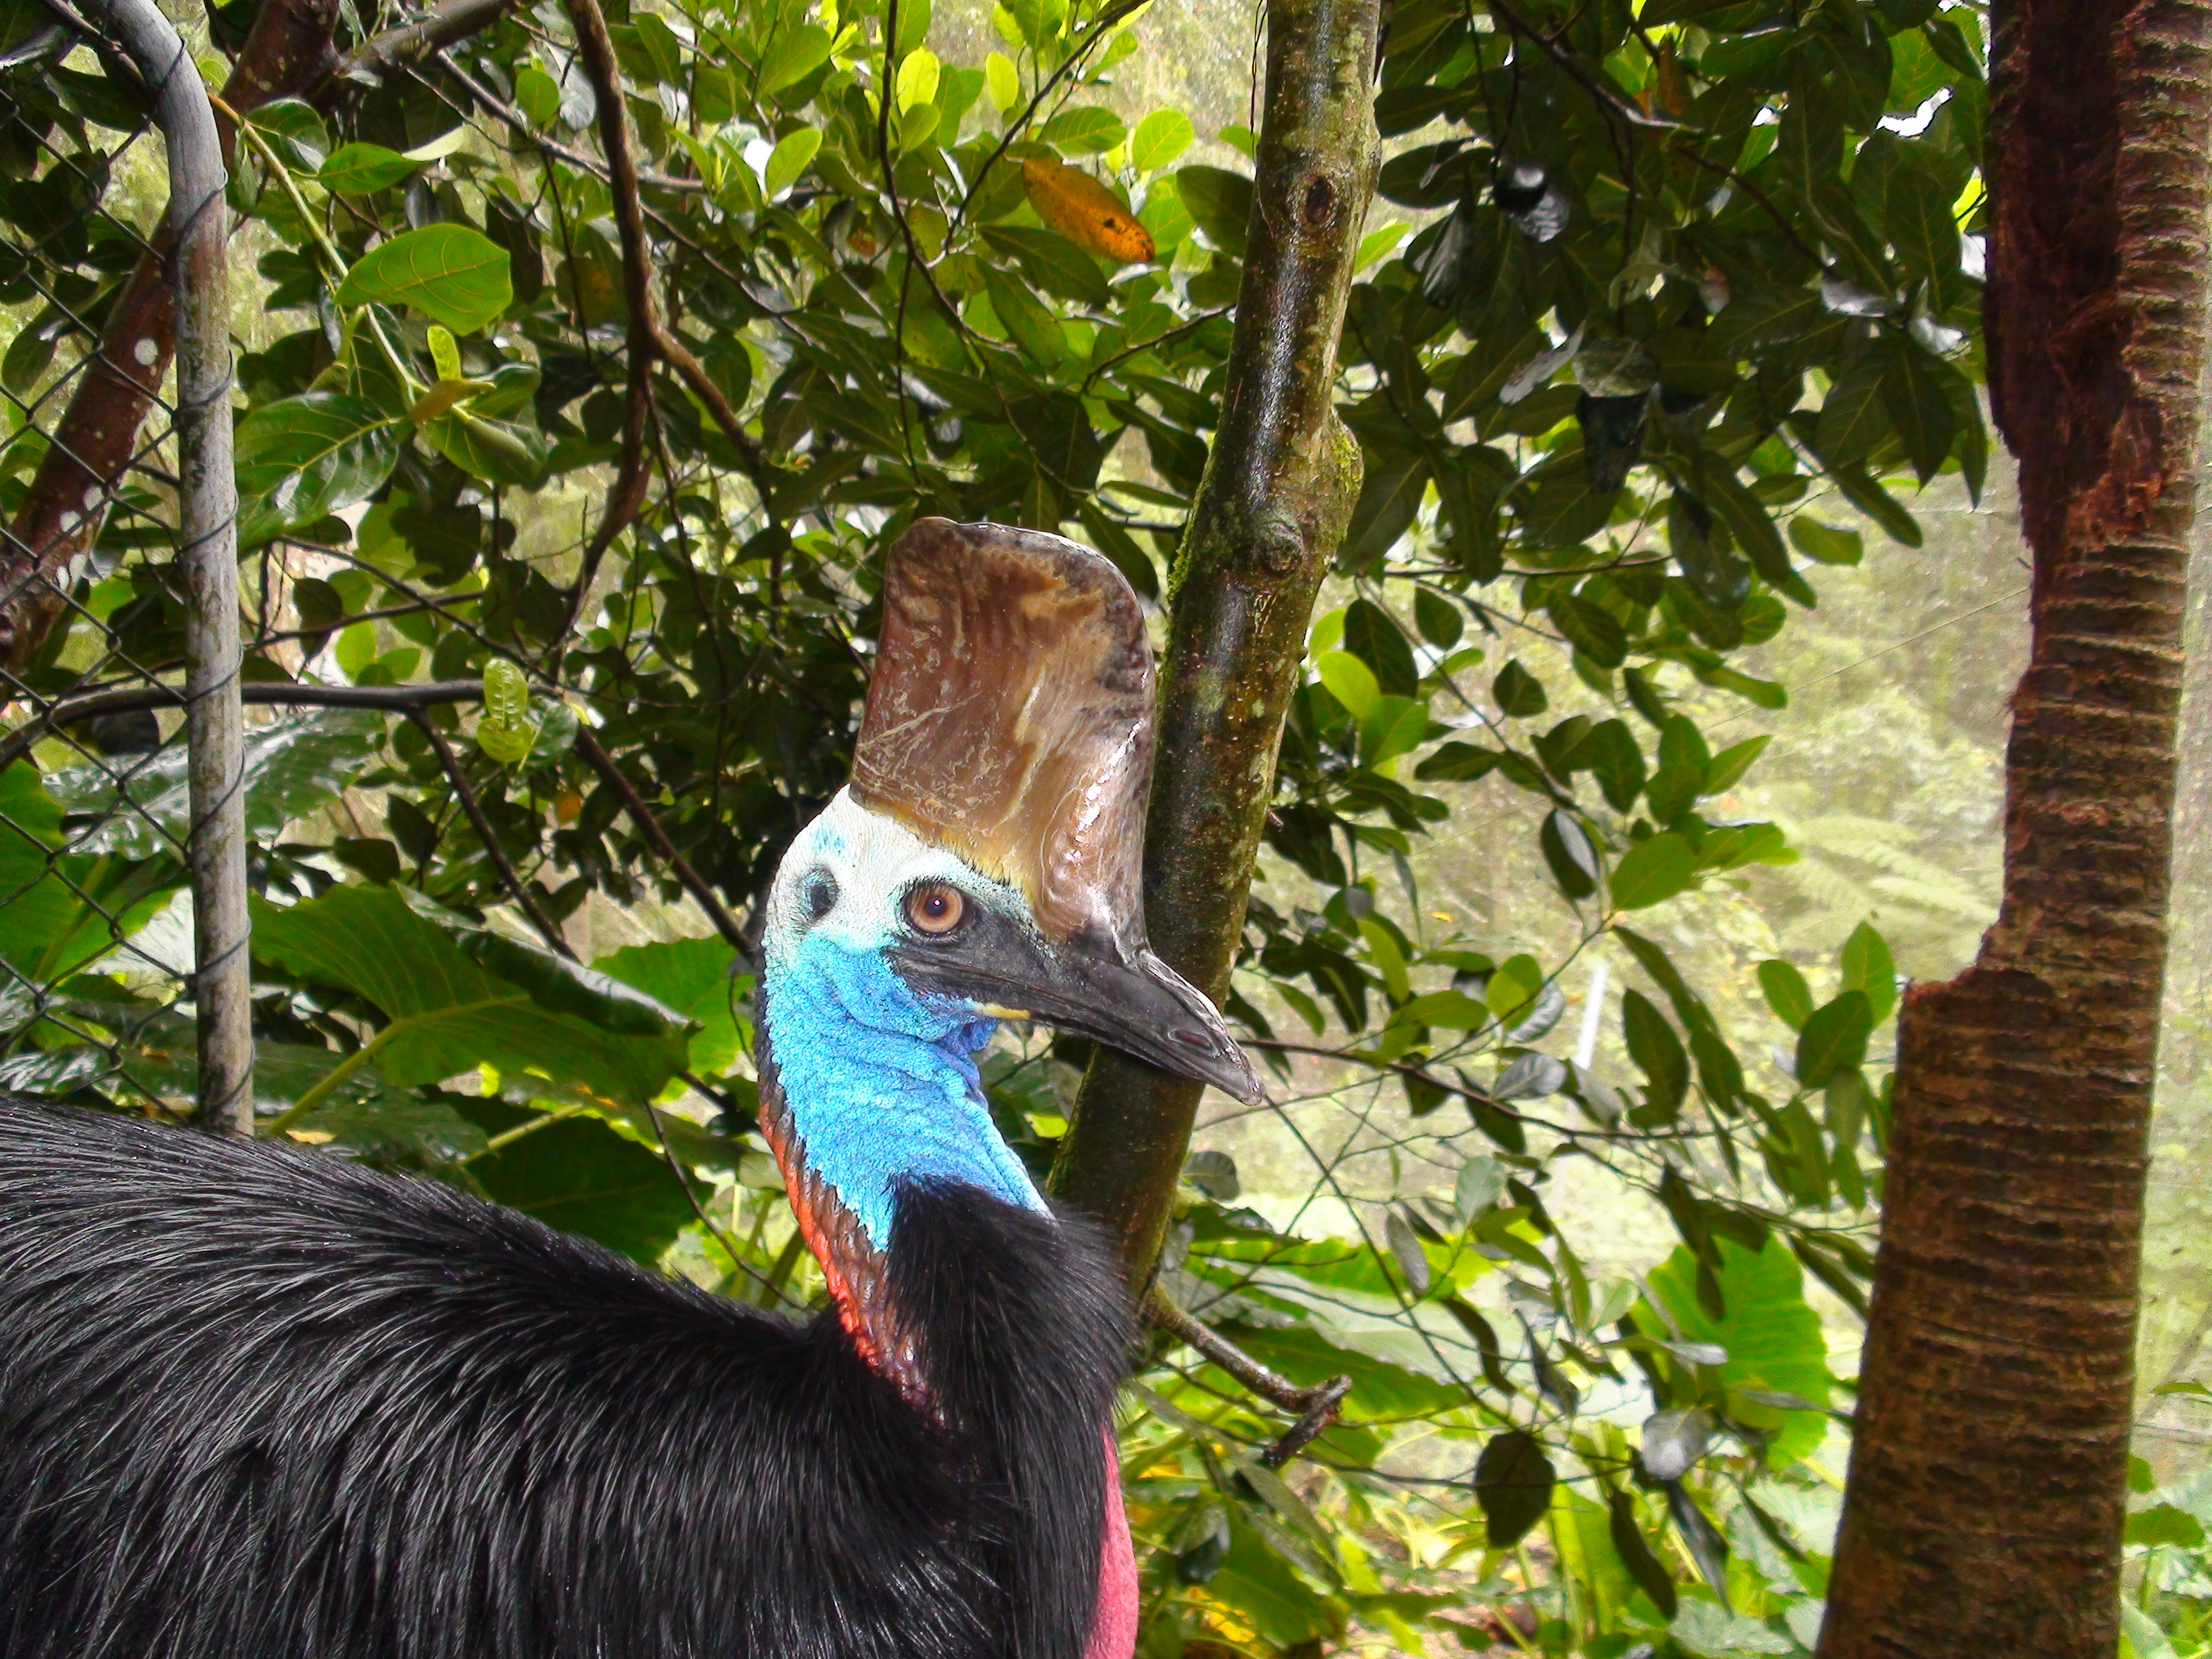
\includegraphics[width=0.4\textwidth]{bird}
}

\quad
\subfloat{
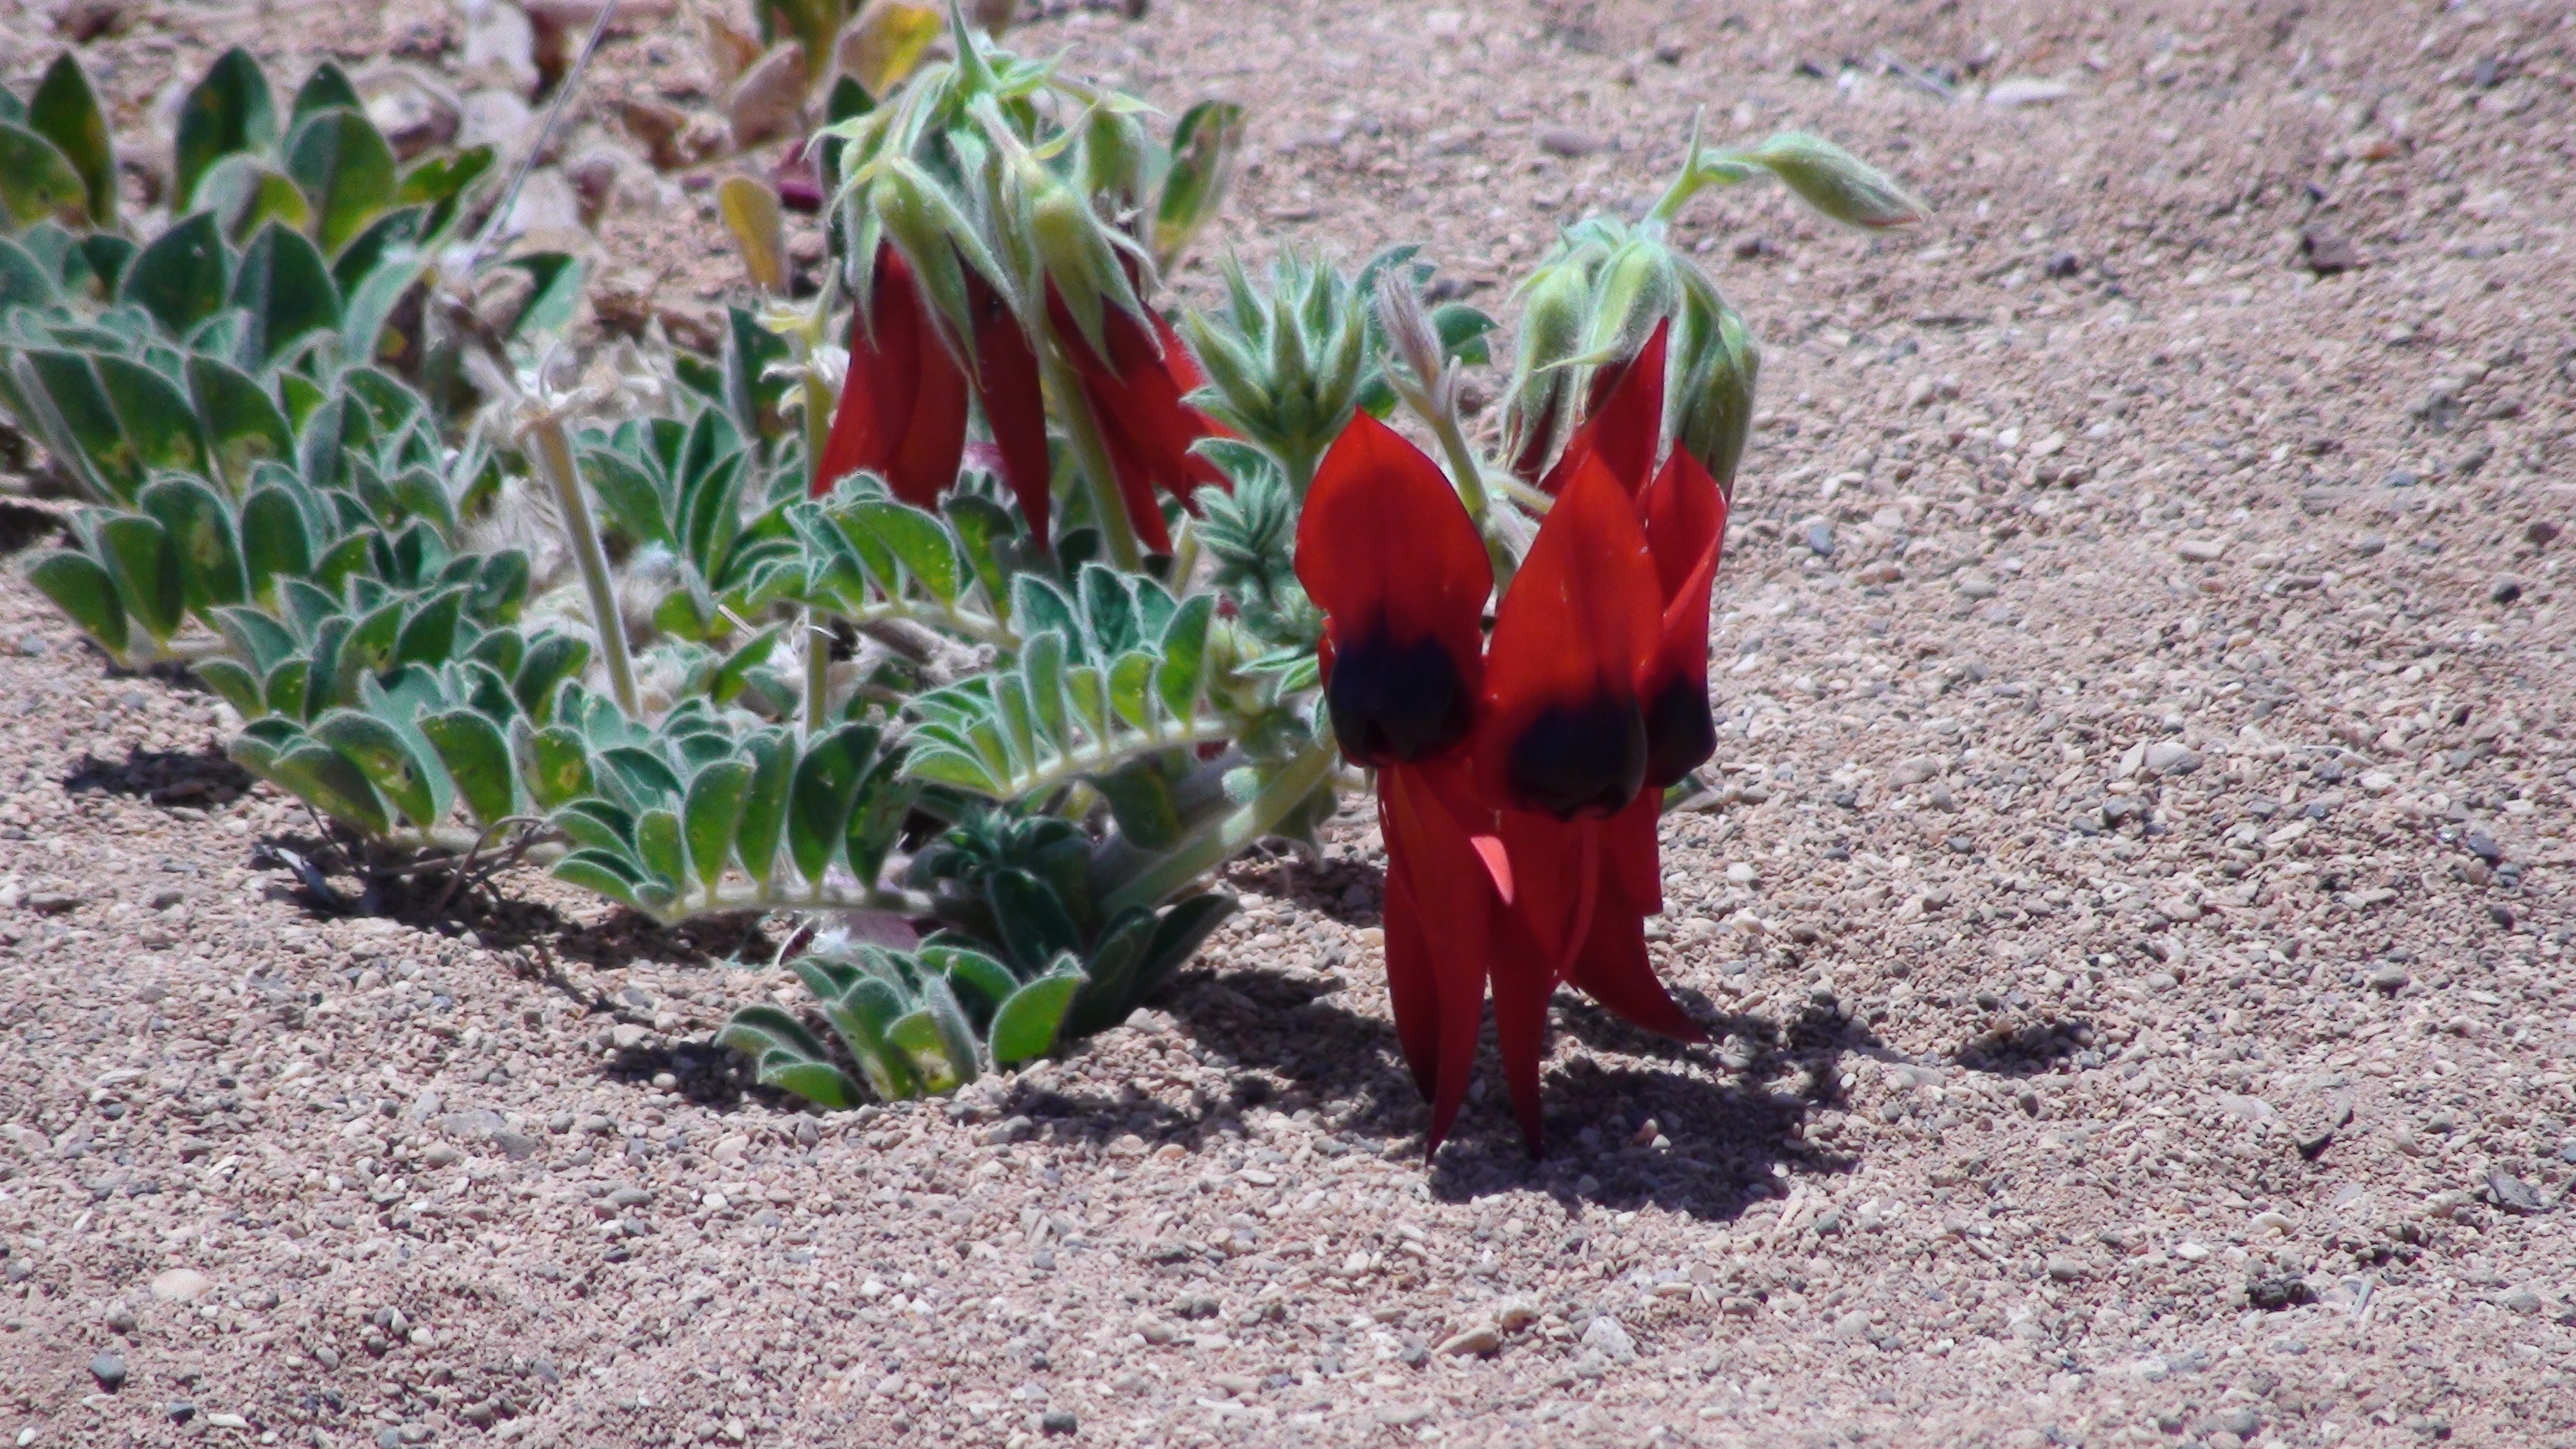
\includegraphics[width=0.4\textwidth]{flower}
}

\quad
\subfloat{
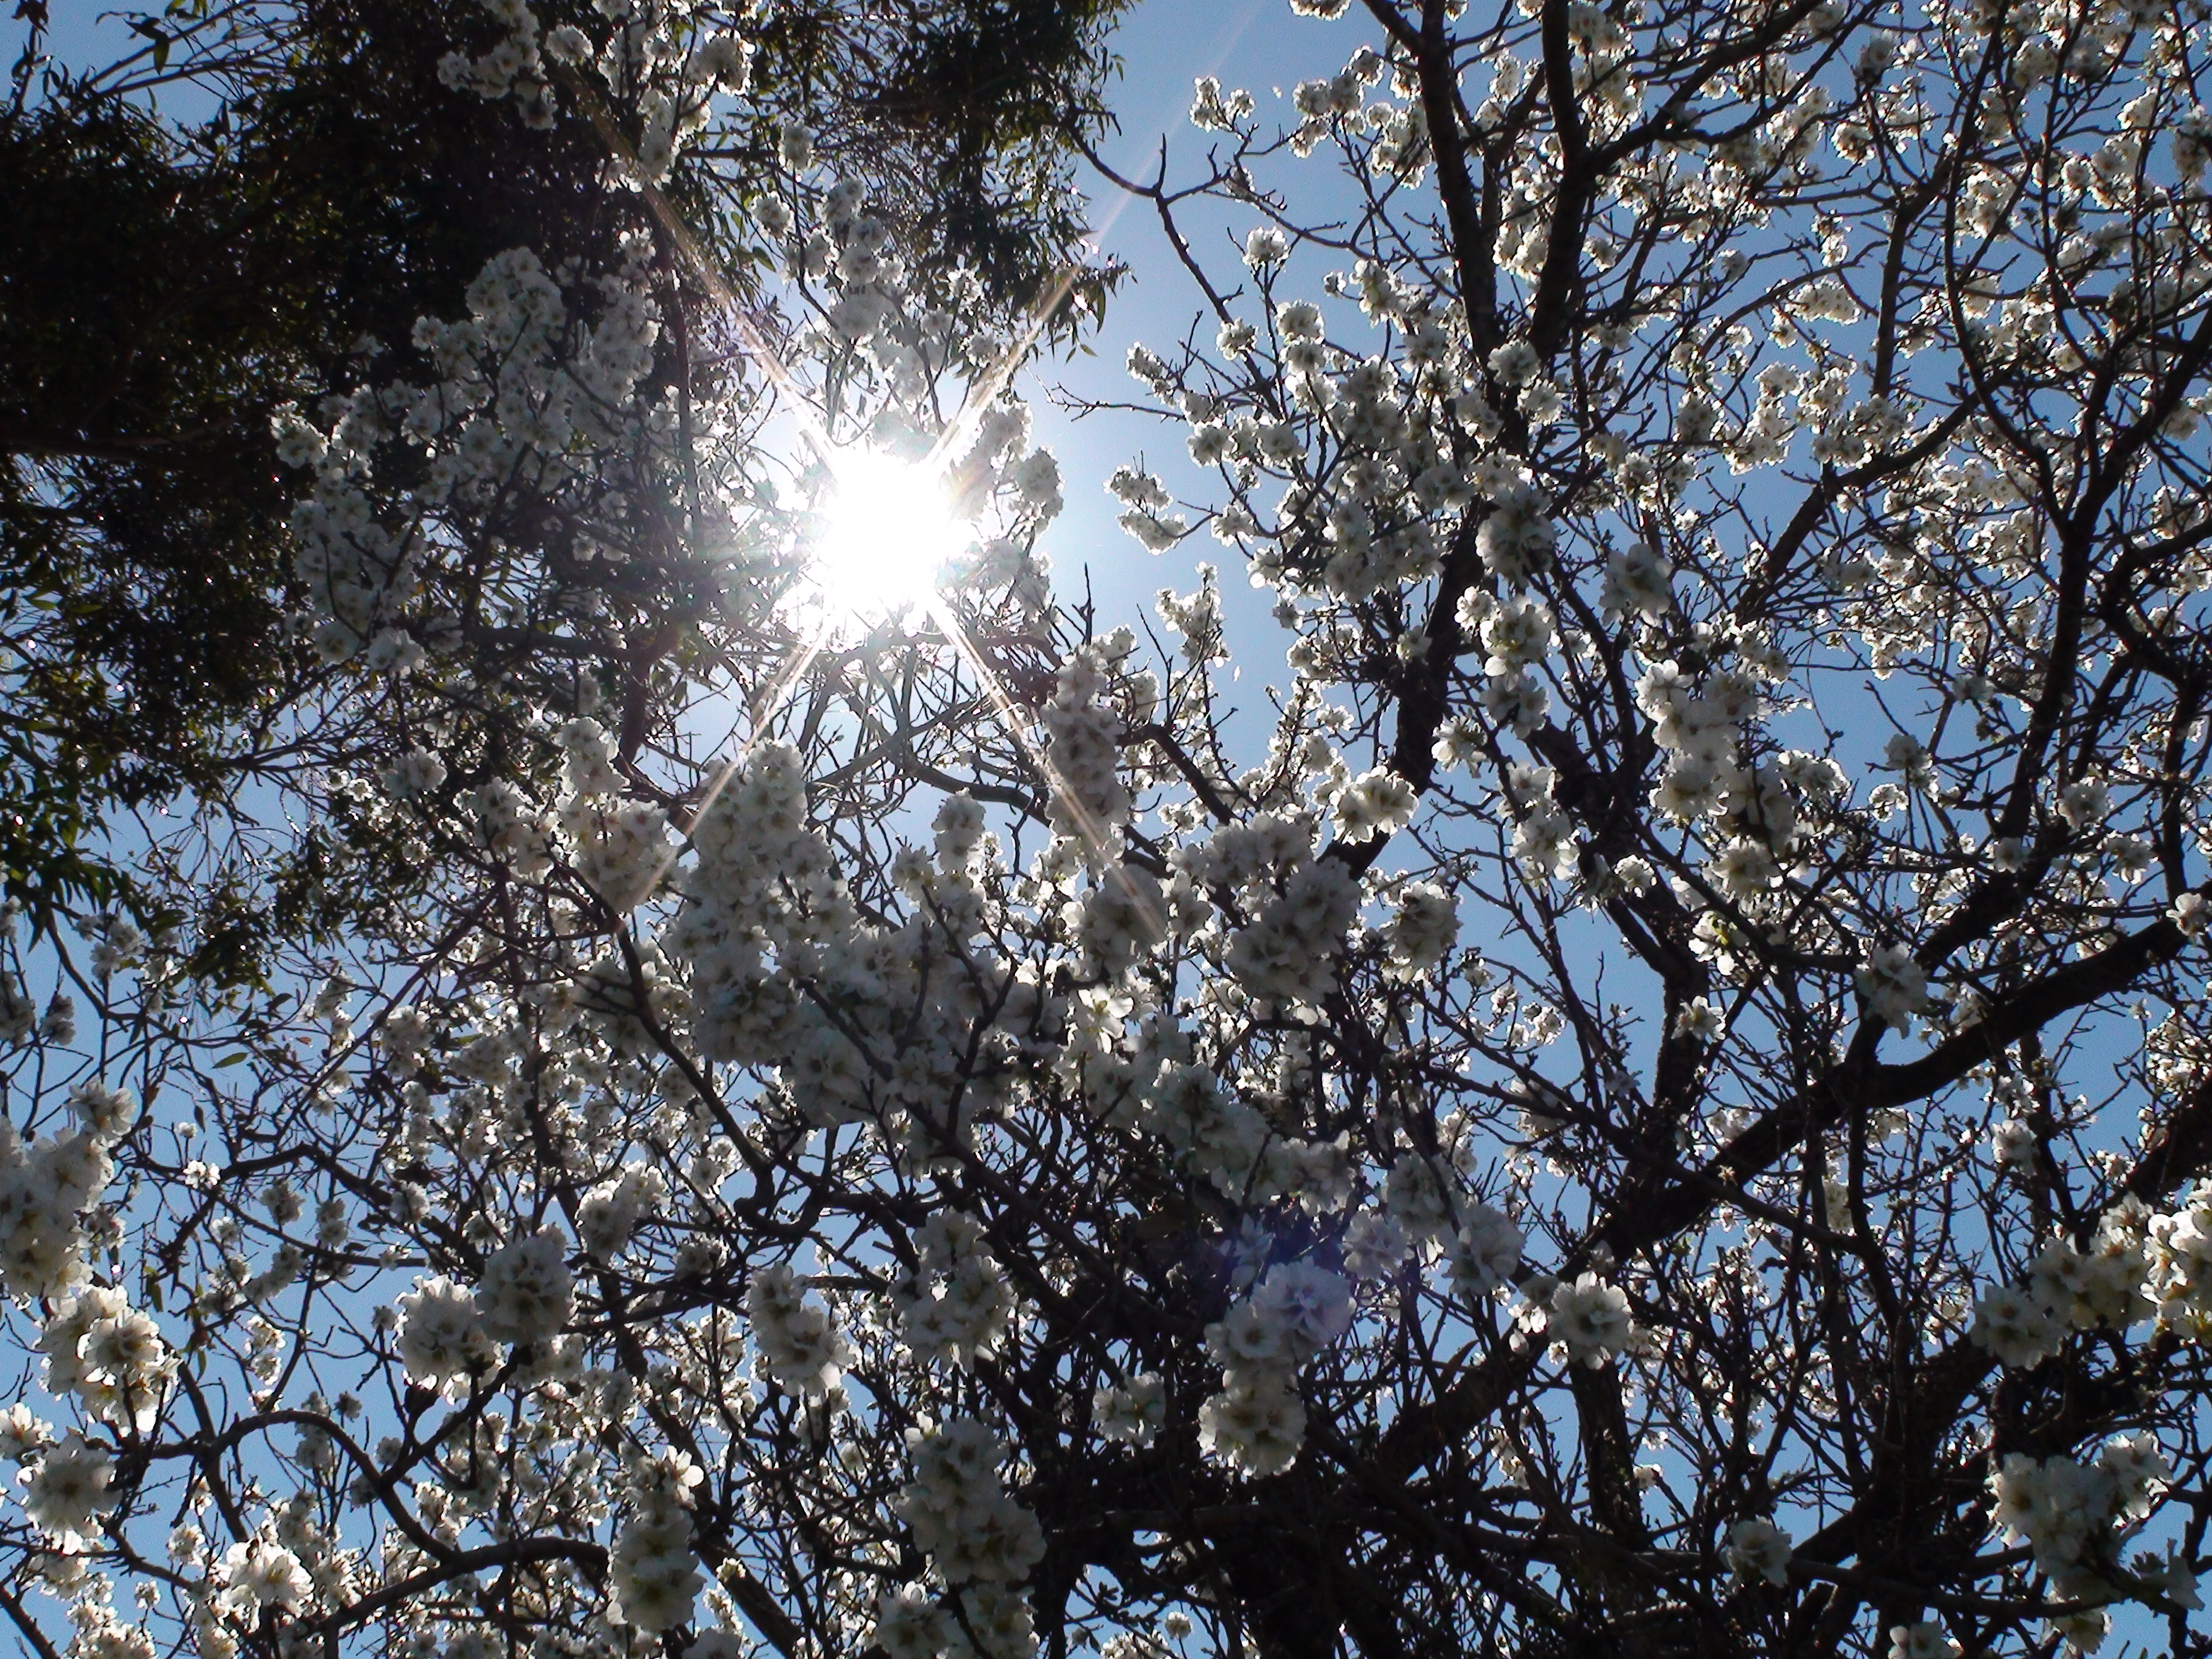
\includegraphics[width=0.4\textwidth]{tree}
}

\caption{This is a bird}
\label{fig:bird}

\end{center}
\end{figure}

\section{Figure}
I have incorporated a figure into my document. To see a cassowary, please see Figure \ref{fig:bird1}
\end{document}
